\documentclass[tikz,border=8pt]{standalone}
\usetikzlibrary{arrows.meta,fit,backgrounds,positioning,calc}
\begin{document}
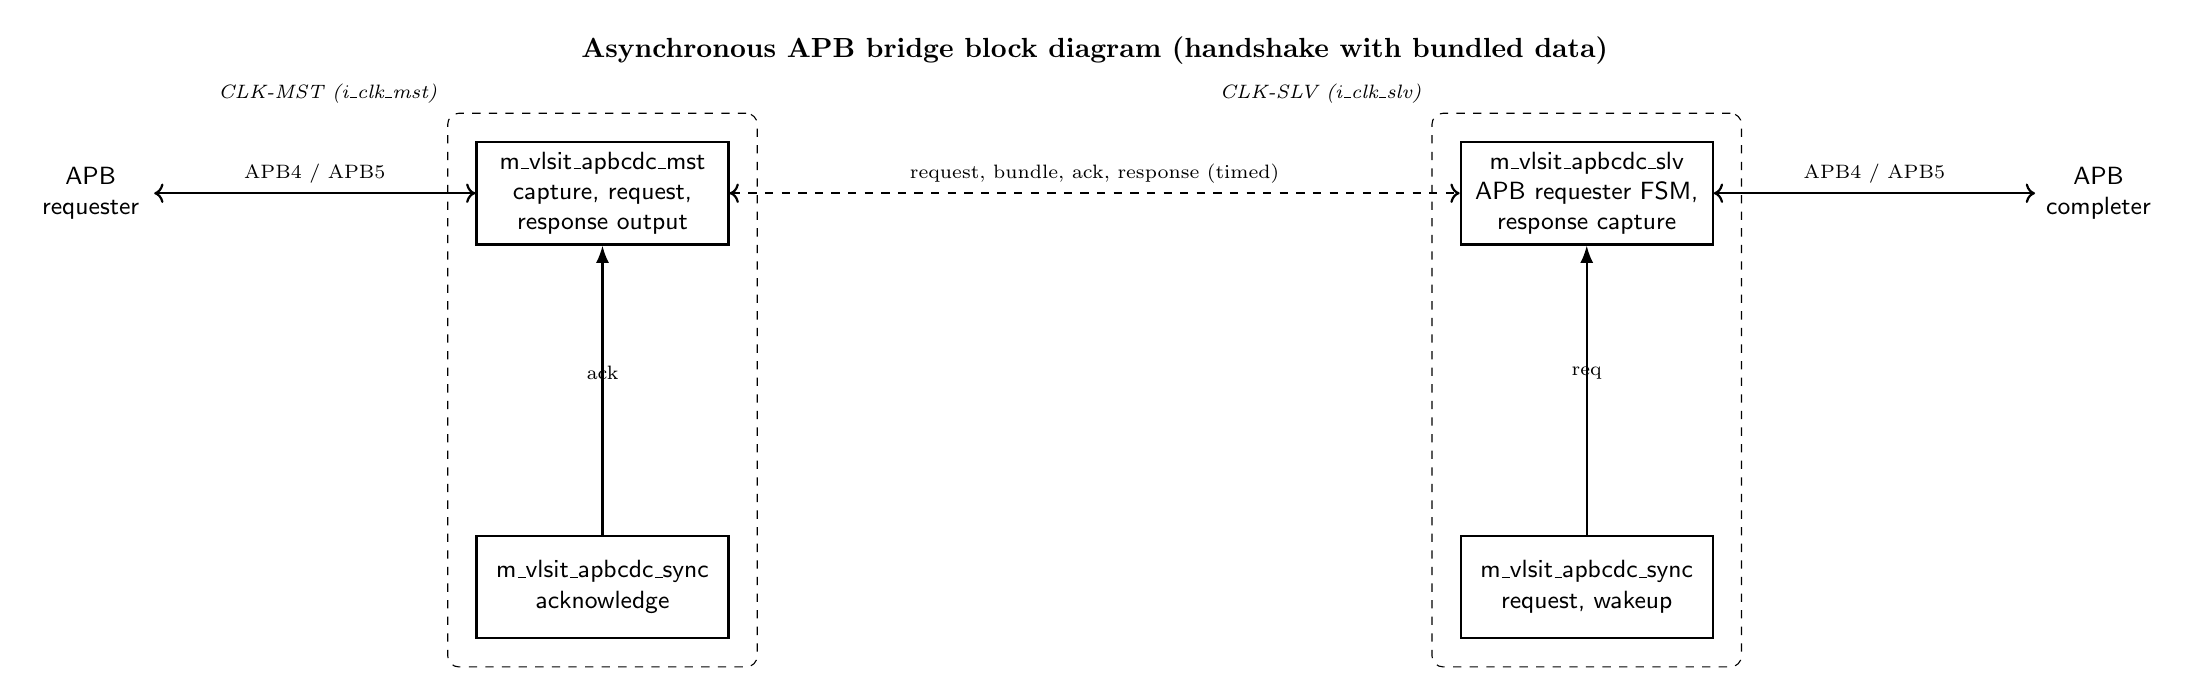
\begin{tikzpicture}[font=\sffamily\small,
  blk/.style={draw,thick,minimum width=3.2cm,minimum height=1.3cm,align=center,fill=white},
  mem/.style={blk,double,double distance=1.5pt},
  clk/.style={blk,rounded corners=6pt},
  io/.style={align=center,minimum width=1.6cm,minimum height=0.8cm},
  data/.style={-{Latex[length=2.2mm]},thick},
  ctrl/.style={-{Latex[length=2.2mm]},thick,dashed},
  clock/.style={-{Latex[length=2.2mm]},thick,dotted}]
\node[io] (io_up) at (0.00,0.00) {APB\\ requester};
\node[blk] (mst) at (6.50,0.00) {m\_vlsit\_apbcdc\_mst\\ capture, request,\\ response output};
\node[blk] (slv) at (19.00,0.00) {m\_vlsit\_apbcdc\_slv\\ APB requester FSM,\\ response capture};
\node[io] (io_dn) at (25.50,0.00) {APB\\ completer};
\node[blk] (sync_a) at (6.50,-5.00) {m\_vlsit\_apbcdc\_sync\\ acknowledge};
\node[blk] (sync_r) at (19.00,-5.00) {m\_vlsit\_apbcdc\_sync\\ request, wakeup};
\draw[data,<->] (io_up.east) -| ($(io_up.east)!.5!(mst.west)$) |- node[midway,above,font=\scriptsize,align=center]{APB4 / APB5} (mst.west);
\draw[ctrl,<->] (mst.east) -| ($(mst.east)!.5!(slv.west)$) |- node[midway,above,font=\scriptsize,align=center]{request, bundle, ack, response (timed)} (slv.west);
\draw[data,<->] (slv.east) -| ($(slv.east)!.5!(io_dn.west)$) |- node[midway,above,font=\scriptsize,align=center]{APB4 / APB5} (io_dn.west);
\draw[data] (sync_a.north) |- ($(sync_a.north)!.5!(mst.south)$) -| node[midway,above,font=\scriptsize,align=center]{ack} (mst.south);
\draw[data] (sync_r.north) |- ($(sync_r.north)!.5!(slv.south)$) -| node[midway,above,font=\scriptsize,align=center]{req} (slv.south);
\begin{scope}[on background layer]
\node[draw,dashed,rounded corners=4pt,inner sep=10pt,fit=(mst)(sync_a),label={[font=\scriptsize\itshape]north west:CLK-MST (i\_clk\_mst)}] (g0) {};
\node[draw,dashed,rounded corners=4pt,inner sep=10pt,fit=(slv)(sync_r),label={[font=\scriptsize\itshape]north west:CLK-SLV (i\_clk\_slv)}] (g1) {};
\end{scope}
\node[font=\bfseries,anchor=south] at (current bounding box.north) {Asynchronous APB bridge block diagram (handshake with bundled data)};
\end{tikzpicture}
\end{document}
